\chapter{Membuat Aplikasi Akademik menggunakan APEX Oracle Online}

\section{Membuat Tabel Data}
Sebelum membuat aplikasi akademik sederhana, buatlah tabel data terlebih dahulu. Ada lima tabel data yang dibuat, yaitu tabel mahasiswa, tabel dosen, tabel kuliah, tabel jadwal, dan tabel nilai. Berikut ini adalah cara membuat tabel data pada APEX Oracle.
\begin{enumerate}
    \item Sig in APEX Oracle online seperti biasa dan masuk ke workspace.
    \item Arahkan kursor ke halaman app builder dan klik from a file
    
\begin{figure}[!htbp]
    \centering
    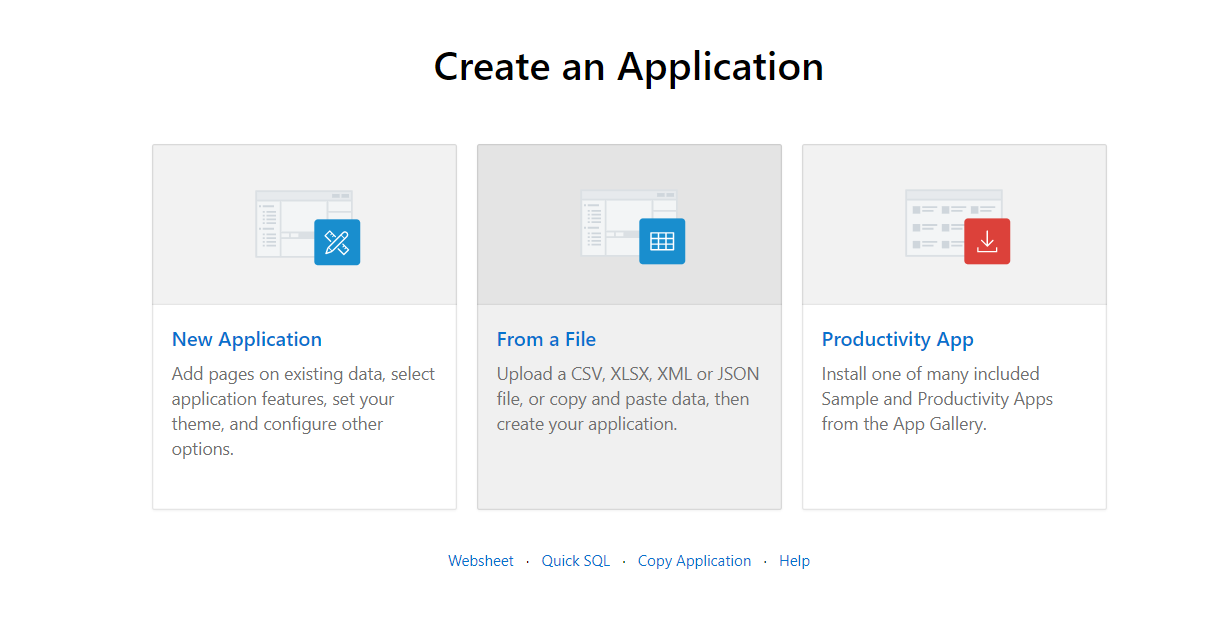
\includegraphics[scale=0.5]{figure/from.png}
    \label{penanda}
\end{figure}  
    
    \item Upload file data excel yang telah dibuat sebelumnya
    \item Buat nama tabel mahasiswa, pilih sheet mahasiswa, dan load data
    
\begin{figure}[!htbp]
    \centering
    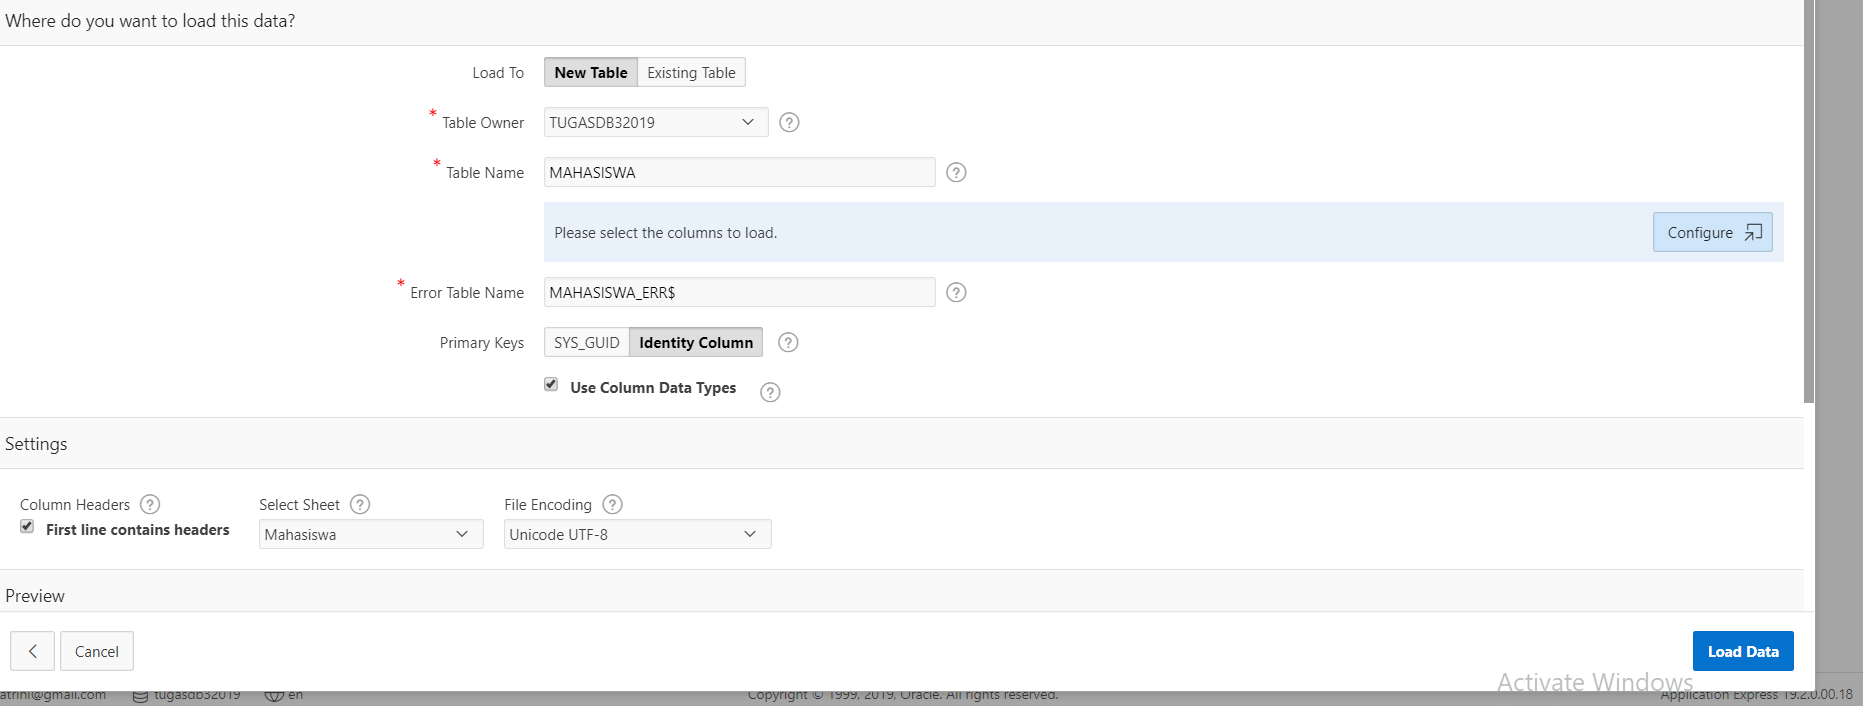
\includegraphics[scale=0.35]{figure/tmhs.png}
    \label{penanda}
\end{figure}  
    
    \item Cara menambahkan tabel yang lainnya tetap sama dengan tabel mahasiswa.
    \item Tabel data mahasiswa berhasil dibuat
\end{enumerate}

\section{Menambahkan Contraints pada Tabel Data}
Pada semua tabel data ditambahkan contraints, yaitu primary key dan foreign key. Berikut ini adalah langkah-langkahnya.
\begin{enumerate}
    \item Sebelum menambahkan contraints, drop column ID pada semua tabel terlebih dahulu.
    \item Klik tabel mahasiswa dan klik contraints
    \item Untuk membuat contraints pilih create
    
\begin{figure}[!htbp]
    \centering
    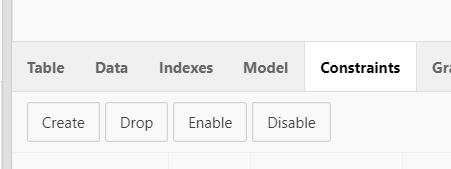
\includegraphics[scale=0.5]{figure/create.png}
    \label{penanda}
\end{figure} 
    
    \item Selanjutnya ubah contraints type menjadi primary key. Lalu, kolom pertama ubah menjadi kolom yang akan diubah menjadi primary, yaitu NIM.
    
\begin{figure}[!htbp]
    \centering
    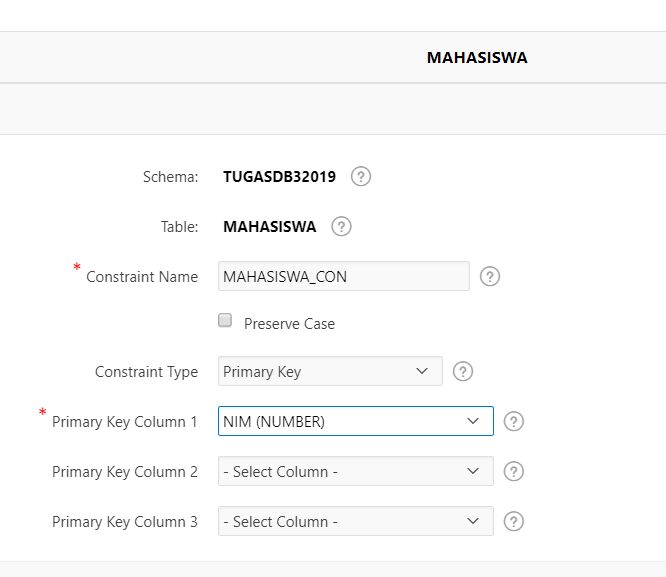
\includegraphics[scale=0.5]{figure/ct.png}
    \label{penanda}
\end{figure} 
    
    \item Langkah-langkah tersebut berlaku untuk menambahkan contraints pada tabel dosen dan kuliah juga.
    \item Setelah itu, menambahkan dua contraints pada tabel jadwal, yaitu dengan kolom NIK dan KODE
    \item Ubah contraints type menjadi foreign key
    \item Pindahkan kolom NIK/KODE disebelah kanan
    \item Pilih referensi tabel dosen/kuliah
    \item Pindahkan kolom NIK/KODE disebelah kanan. Lalu klik next dan finish.
    \item Lalu, buat contraints satu lagi NIK/KODE, langkah-langkahnya sama dengan cara diatas
    
\begin{figure}[!htbp]
    \centering
    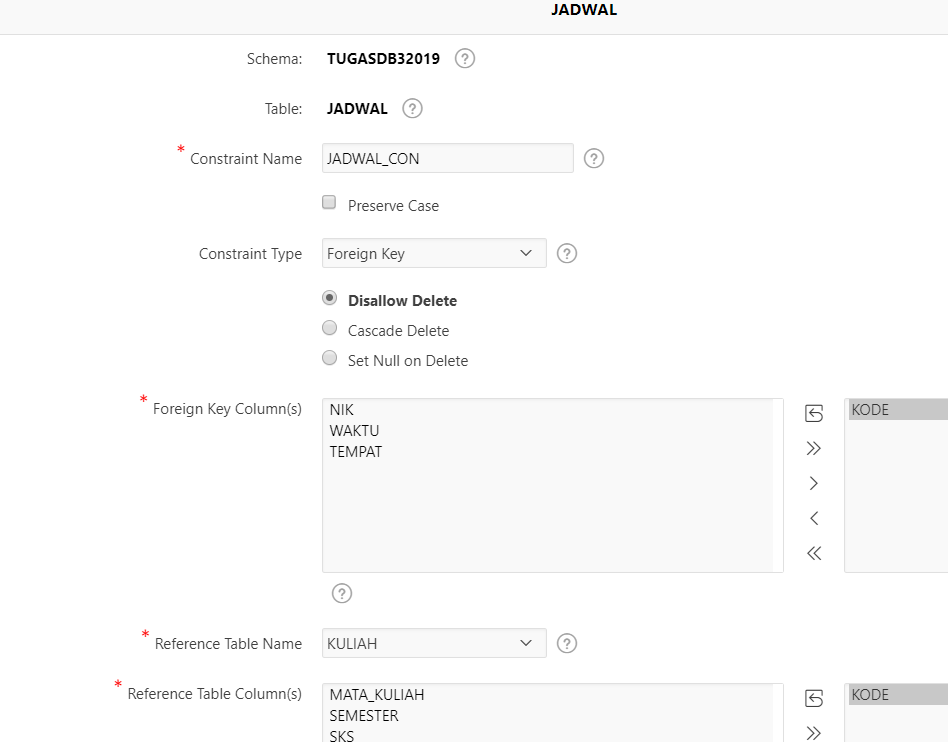
\includegraphics[scale=0.5]{figure/cjd.png}
    \label{penanda}
\end{figure} 
    
    \item Selanjutnya menambahkan dua contraints juga pada tabel nilai, yaitu KODE dan NIM
    \item Caranya sama dengan menambahkan contraints pada tabel jadwal
    
\begin{figure}[!htbp]
    \centering
    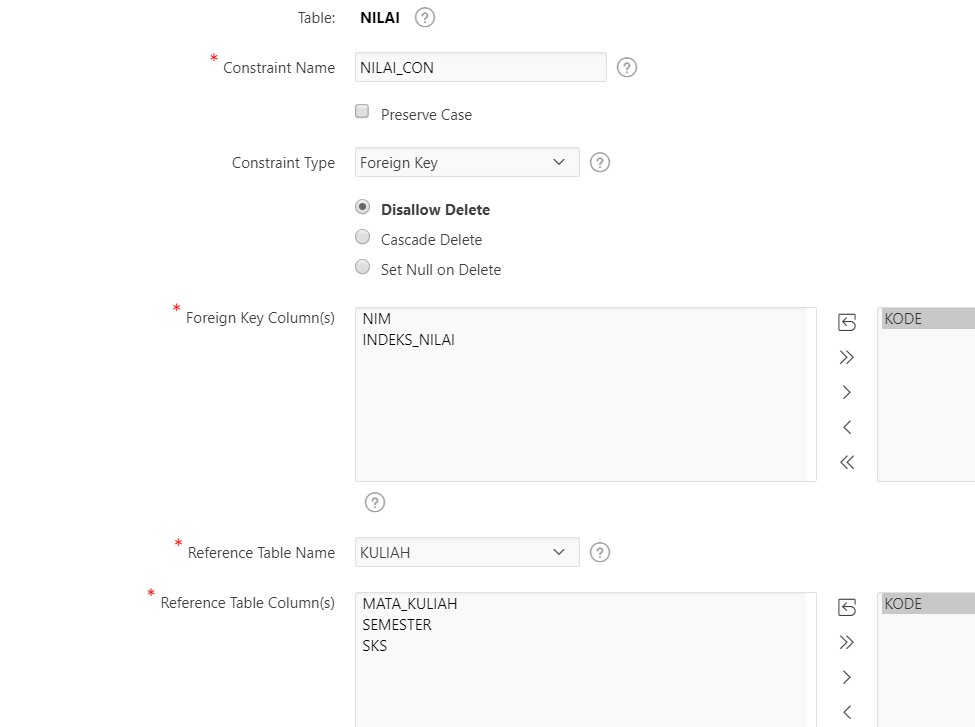
\includegraphics[scale=0.5]{figure/cjd2.png}
    \label{penanda}
\end{figure}     
  
  \item Menambahkan contraints pada semua tabel telah selesai
    
\end{enumerate}

\section{Membuat Aplikasi Akademik Sederhana}
Setelah melakukan semua langka-langkah diatas, selanjutnya adalah membuat aplikasinya. 

\begin{enumerate}
    \item Sebelum membuat aplikasi, aturlah terlebih dahulu page yang di inginkan. Berikut ini adalah page yang ditambahkan pada aplikasi akademik sederhana.

\begin{figure}[!htbp]
    \centering
    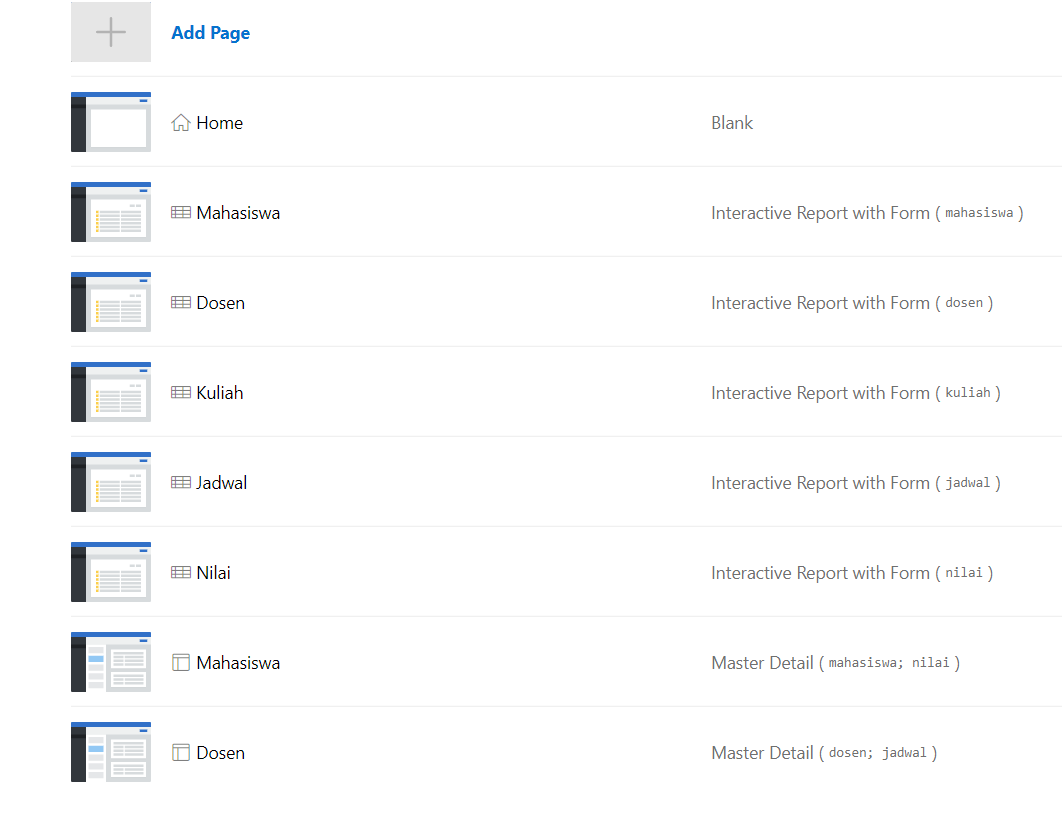
\includegraphics[scale=0.4]{figure/page.png}
    \label{penanda}
\end{figure}

    \item Selanjutnya adalah klik create aplikasi yang akan dibuat. Aplikasi akan loading sebentar. Setelah aplikasi selesai dibuat, tampilannya akan seperti gambar dibawah ini.
    
\begin{figure}[!htbp]
    \centering
    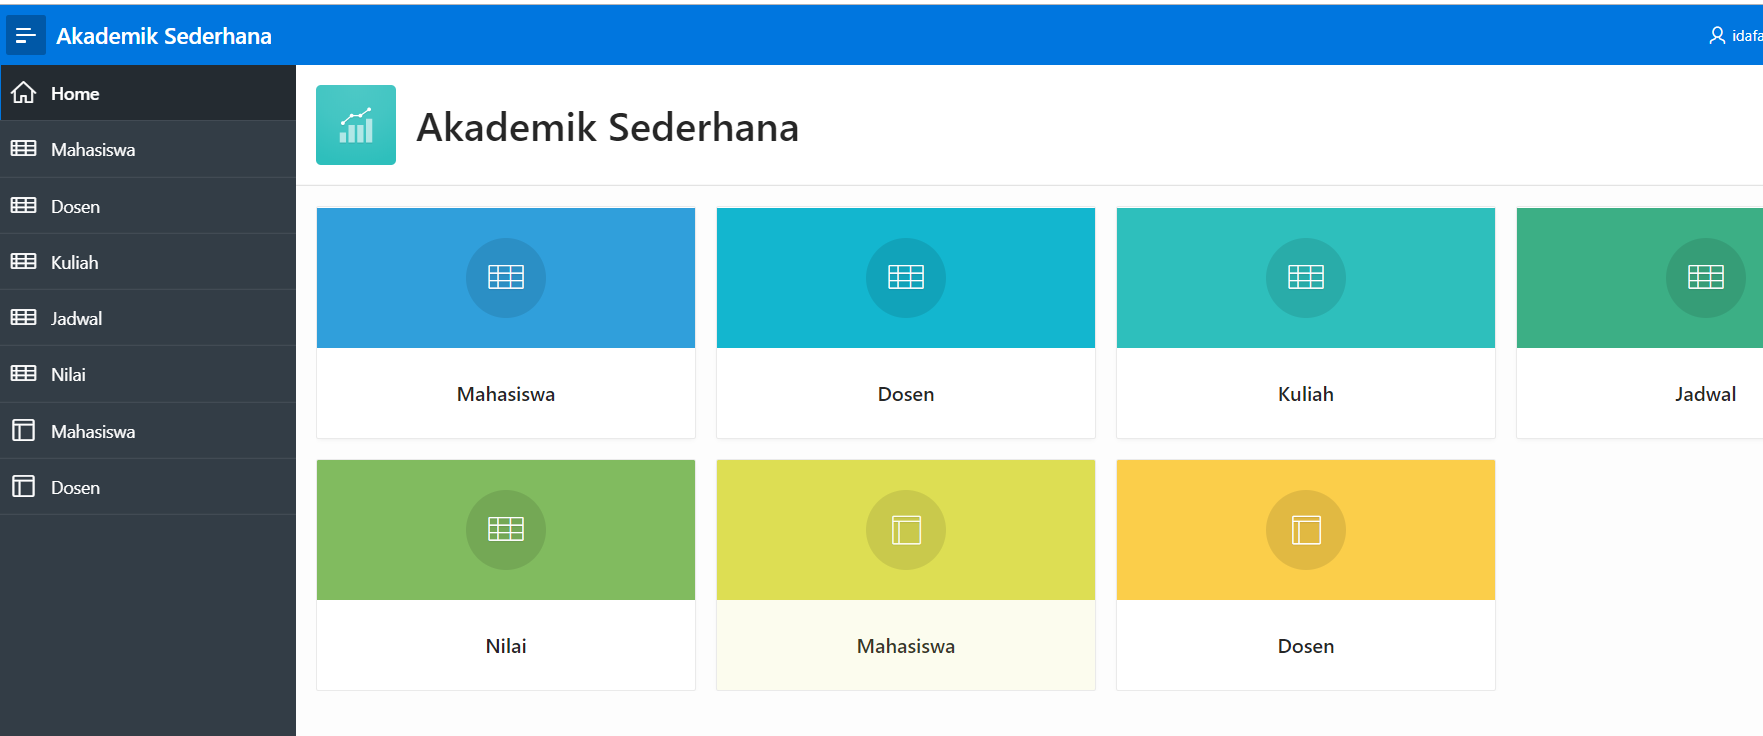
\includegraphics[scale=0.35]{figure/as.png}
    \label{penanda}
\end{figure}
    
\end{enumerate}

- link: https://apex.oracle.com/pls/apex/f?p=93546:LOGIN_DESKTOP:708969285882655:::::

- email: idafatrini@gmail.com 

- pass: sayangdia123